% --- CHƯƠNG 4: THỐNG KÊ ---
\chapter{Trực quan hóa dữ liệu thống kê}
Để có cái nhìn tổng quan về kết quả review, dữ liệu lỗi đã được tổng hợp và trực quan hóa bằng Python.

\begin{figure}[htbp]
  \centering
  % Cập nhật đường dẫn hình ảnh
  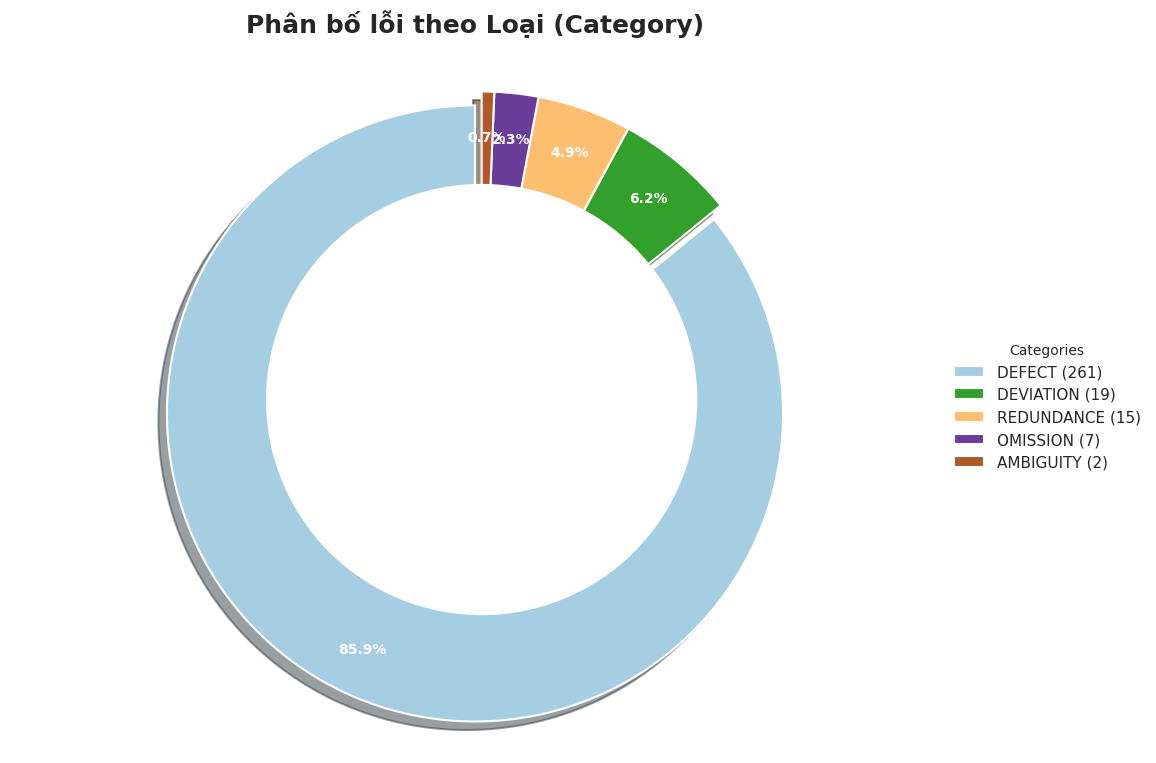
\includegraphics[width=0.9\textwidth]{images/bieu_do_pie_category.png}
  \caption{Tỷ lệ phân bố lỗi theo 5 loại chính (Category). Đa số lỗi thuộc nhóm DEFECT (khiếm khuyết trong logic).}
  \label{fig:pie_chart}
\end{figure}

\begin{figure}[htbp]
  \centering
  % Cập nhật đường dẫn hình ảnh
  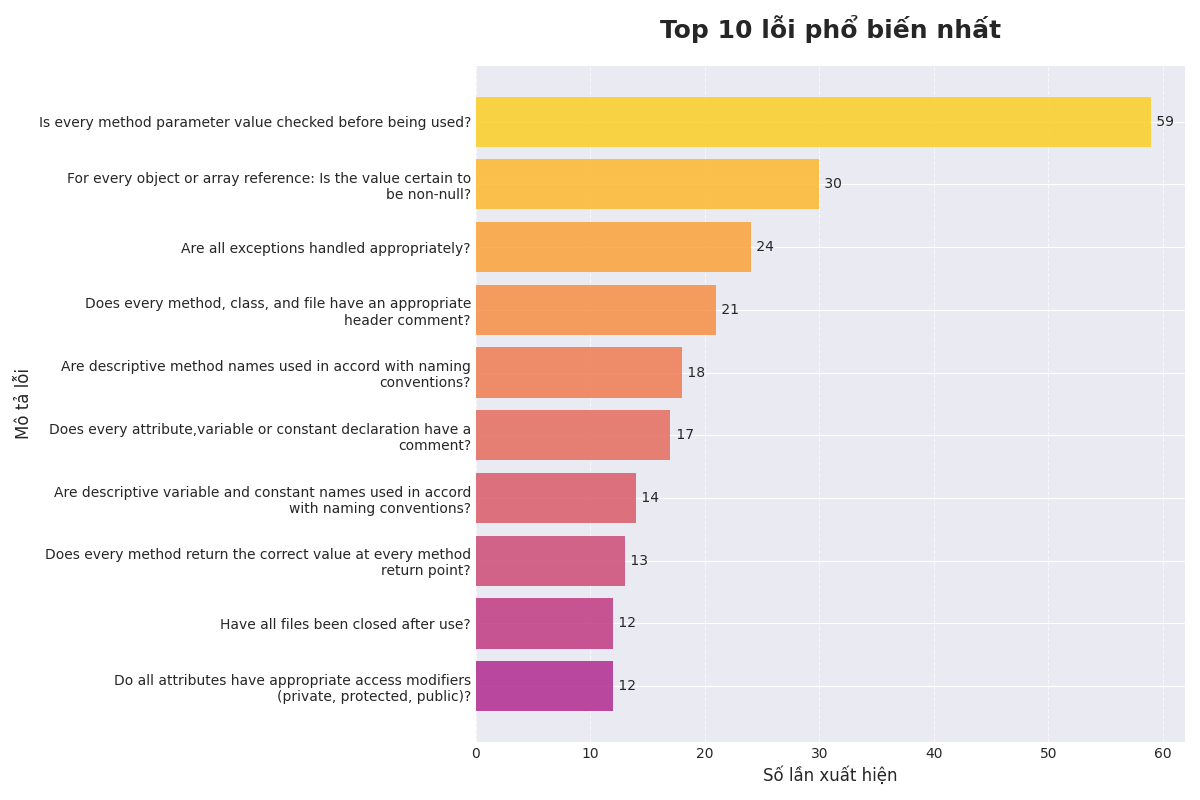
\includegraphics[width=1\textwidth]{images/bieu_do_top_10_loi.png}
  \caption{Top 10 lỗi phổ biến nhất. Lỗi "thiếu kiểm tra tham số" (Mã 15) là phổ biến nhất và cũng là nguyên nhân chính gây ra lỗi SQL Injection.}
  \label{fig:top10_chart}
\end{figure}

\begin{figure}[htbp]
  \centering
  % Cập nhật đường dẫn hình ảnh
  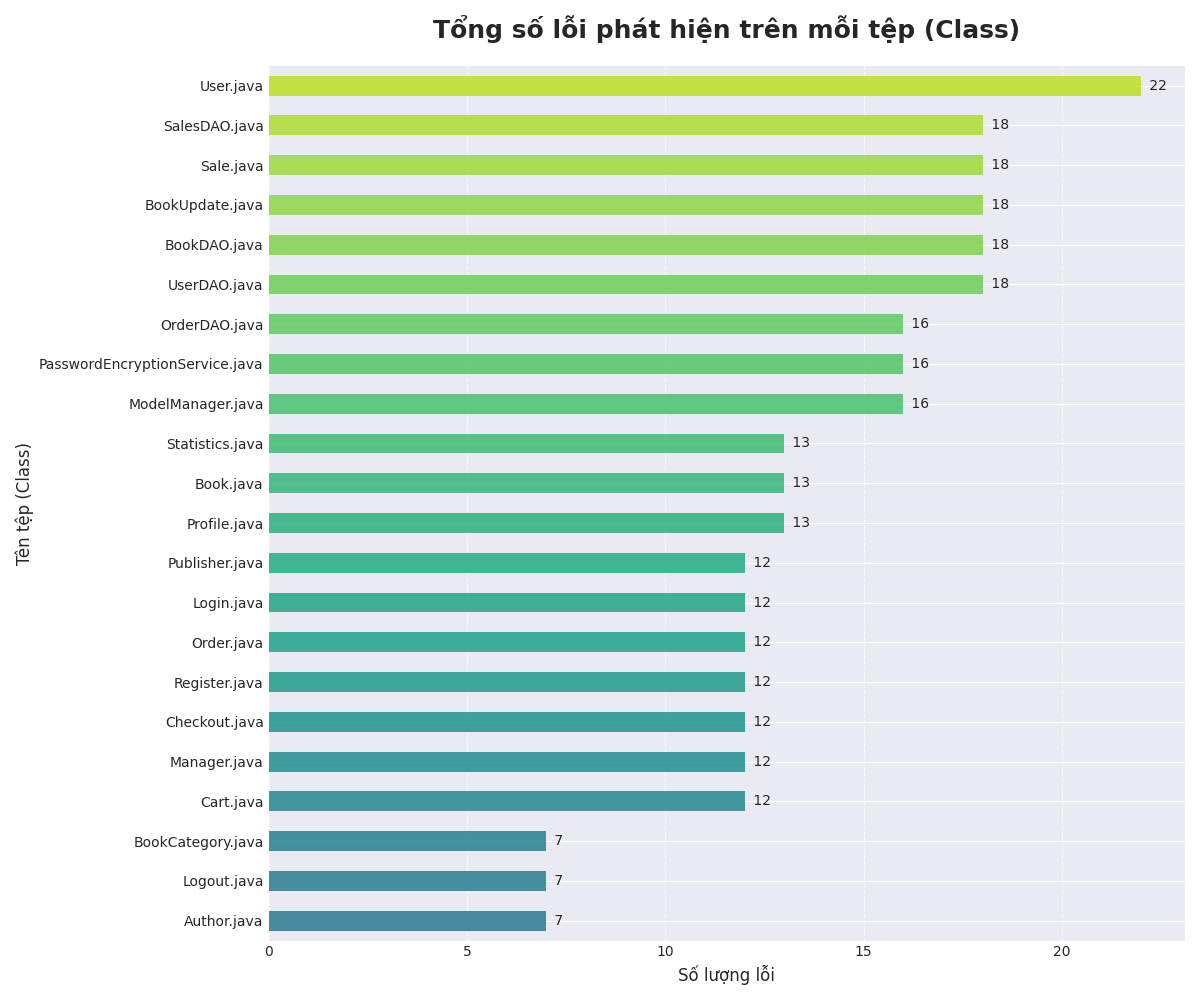
\includegraphics[width=1\textwidth]{images/bieu_do_loi_moi_tep.png}
  \caption{Phân bố số lượng lỗi trên từng tệp. \texttt{BookDAO.java} và \texttt{BookUpdate.java} là hai file có nhiều vấn đề nhất.}
  \label{fig:files_chart}
\end{figure}

\begin{figure}[htbp]
  \centering
  % Cập nhật đường dẫn hình ảnh
  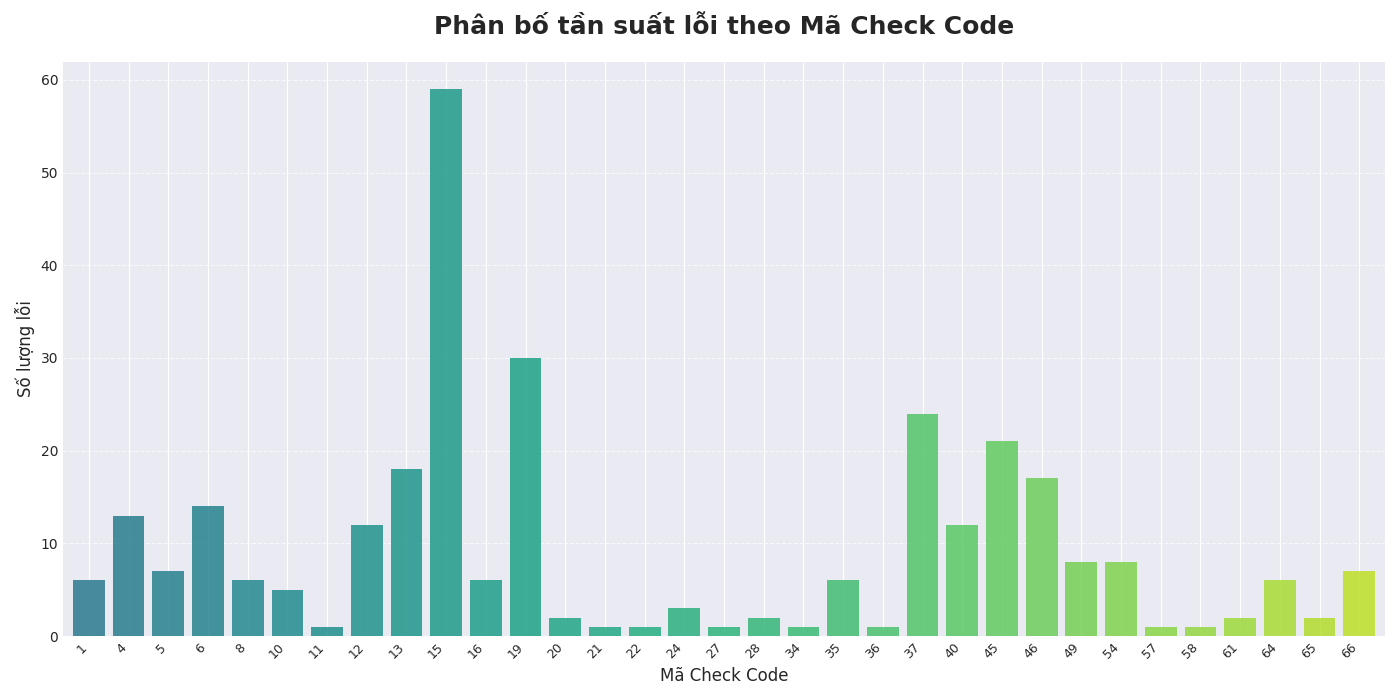
\includegraphics[width=1\textwidth]{images/bieu_do_phan_bo_loi.png}
  \caption{Tần suất xuất hiện của từng mã lỗi (Check code).}
  \label{fig:checkcode_chart}
\end{figure}

\newpage